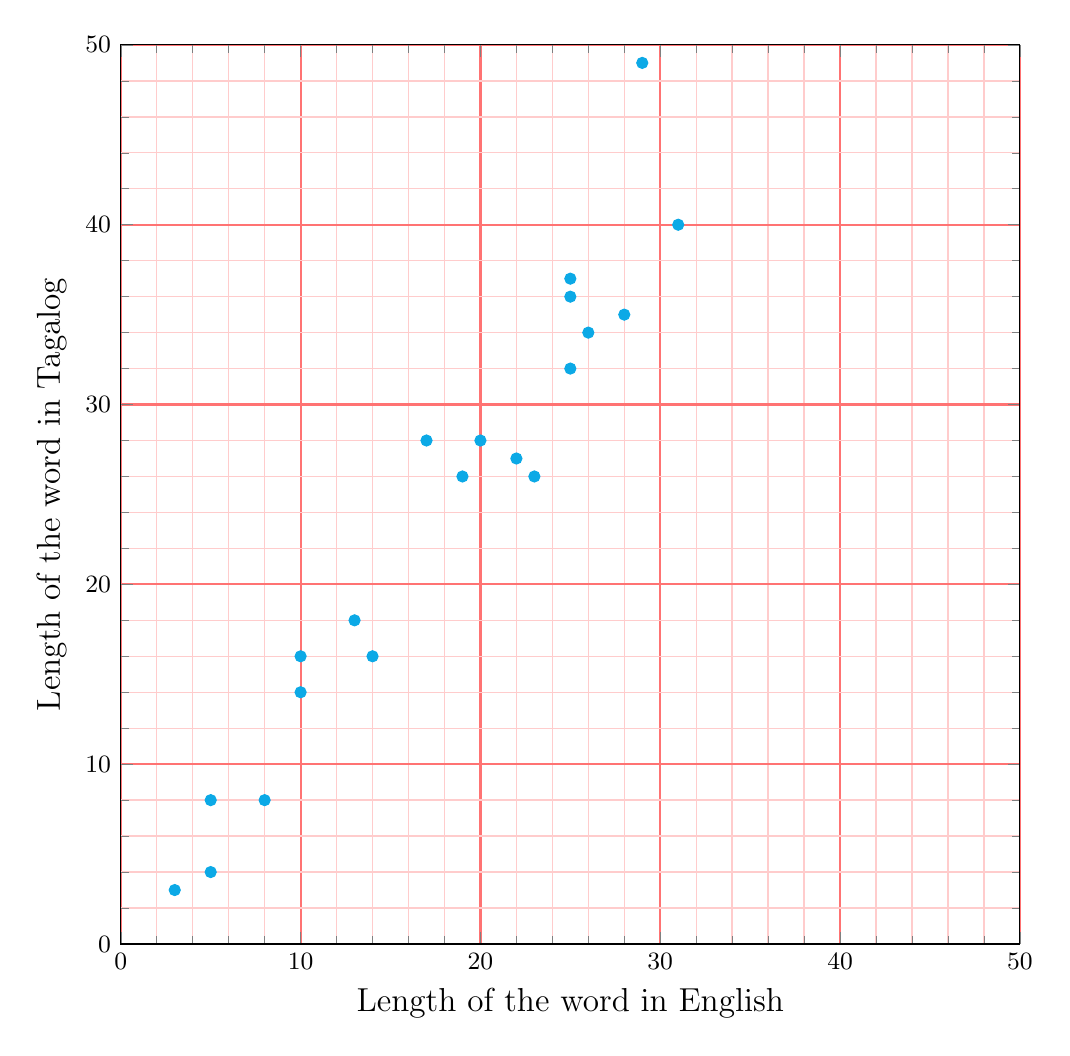
\begin{tikzpicture}
\begin{axis}[
    width=13cm, height=13cm,
    xlabel={Length of the word in English},
    ylabel={Length of the word in Tagalog},
    xmin=0, xmax=50,
    ymin=0, ymax=50,
    xtick={0,10,20,30,40,50},
    ytick={0,10,20,30,40,50},
    minor tick num=4,              % 4 minor ticks, so 5 cells and 2-unit minor grid
    grid=both,
    major grid style={red!55, line width=0.8pt},
    minor grid style={red!20, line width=0.5pt},
    axis lines=box,
    tick align=inside,
    xlabel style={font=\large},
    ylabel style={font=\large},
    tick label style={font=\small},
    ]

    \addplot[
    only marks,
    mark=*,
    mark size=2pt,
    color=cyan!95!black,
    ] coordinates {
    (3,3)  (5,4)  (5,8)  (8,8) (10,14) (10,16) (13,18) (14,16)
    (17,28) (19,26) (20,28) (22,27) (23,26) (25,32) (25,36) 
    (25,37) (26,34) (28,35) (29,49) (31,40)
    };

\end{axis}
\end{tikzpicture}